\section{1174039 - Liyana Majdah Rahma}
        \subsection{Teori}
            \subsubsection{Definisi Kecerdasan Buatan}

            Artificial Inteligence adalah kecerdasan yang ditambahkan  pada suatu sistem yang dapat diatur dalam konteks secara ilmiah. Menurut Michael Haelein menyatakan bahwa  AI meupakan “sistem yang mempunyai kemampuan untuk menguraikan, belajar agar dapat dugunakan untuk mencapai tujuan dengan melalui adaptasi yang fleksibel”. Kecerdasan buatan juga dapat dibuat dan dimasukkan ke dalam mesin agar dapat melakukan pekerjaan seperti yang dapat dilakukan manusia dengan cepat dan tepat. 
            
            \subsubsection{Sejarah Kecerdasan Buatan}

            Sejarah Kecerdasan buatan pertama kali terjadi pada zaman kuno, terdapat mitos ataupun cerita dan desas-desus tentang sebuah mahkluk yang mempunyai kecerdasan serta kesadaran yang diberikan oleh pengrajin. Benih - benih nya mulai ditanam oleh para filsuf klasik yang mencari cara untuk menggambarkan proses berfikir manusia sebagai manipulasi simbol secara mekanis yang memuncak pada penemuan komputer digital di tahun 1940-an, yaitu sebuah mesin yang didasarkan penalaran matematika. Istilah kecerdasan buatan sendiri baru muncul pada tahun 1956, dan teori -teori nya sudah muncul sejak tahun 1941. Dan Pada tahun 1973, sebagai tanggapan atas kritik dari James Lighthill dan tekanan terus-menerus dari kongres, AS dan Pemerintah Inggris menghentikan pendanaan penelitian yang tidak diarahkan pada kecerdasan buatan, dan tahun-tahun sulit berikutnya akan dikenal sebagai musim dingin AI. Tujuh tahun kemudian, sebuah inisiatif visioner oleh Pemerintah Jepang mengilhami pemerintah dan industri untuk menyediakan miliaran dolar dalam AI, tetapi pada akhir 80-an investor menjadi kecewa dengan kurangnya daya komputer (perangkat keras) yang dibutuhkan dan menarik lebih banyak dana.

            \subsubsection{Perkembangan Kecerdasan Buatan}
            \begin{enumerate}
                \item Pada tahun 1958, McCarthy di MIT AI Lab Memo orang pertama yang mendefinisikan bahasa pemrograman pada tingkat tinggi yaitu LISP, yang sekarang mendominasi pembuatan program-pogram kecerdasan buatan.
                \item Kemudian Pada tahun 1959, Nathaniel Rochester dari IBM serta mahasiswa-mahasiswanya mengeluarkan program kecerdasan buatan yaitu Geometry Theorm Prover. selain itu juga Program ini dapat mengeluarkan suatu teorema menggunakan aksioma-aksioma yang ada.
                \item Sistem Berbasis Pengetahuan pada tahun 1969-1979
                \item  Kecerdasan Buatan menjadi sebuah industri pada tahun 1980-1988. Kembalinya Jaringan Syaraf tiruan pada tahun 1986-sekarang.
            \end{enumerate}
            \subsection{Instalasi}
            \subsubsection{Instalasi Library Scikit dari Anaconda}
            \begin{enumerate}
                \item Download aplikasi Anaconda terlebih dahulu. 
                \item Install aplikasi Anaconda yang sudah di download tadi. 
                \item Simpan aplikasi sesuai folder yang kita pilih lalu next. 
                \item Centang Keduanya lalu tekan tombol install. 
                \item Setelah itu tunggu sampai proses instalasi selesai lalu jika sudah tekan tombol finish. 
                \item Lalu buka command prompt anda dan tuliskan perintah berikut ini untuk mengecek apakah aplikasinya sudah   terinstall. 
                \item Kemudian ketikkan perinta pip install -U scikit-learn seperti gambar berikut. 
            \end{enumerate}
             \begin{figure}[H]
                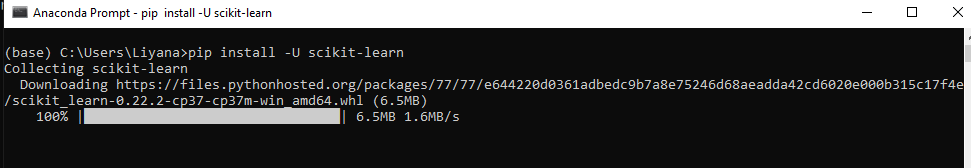
\includegraphics[width=4cm]{figures/1174039/chaptersatu/1.png}
                \centering
                \caption{Instalasi}
            \end{figure}
            \item Pilih salah satu example dari website tersebut lalu jalankan \hfill \break \lstinputlisting[firstline=1]{src/1174039/chaptersatu/no1.py}
                \item buka variable explolernya
                \begin{figure}[H]
                    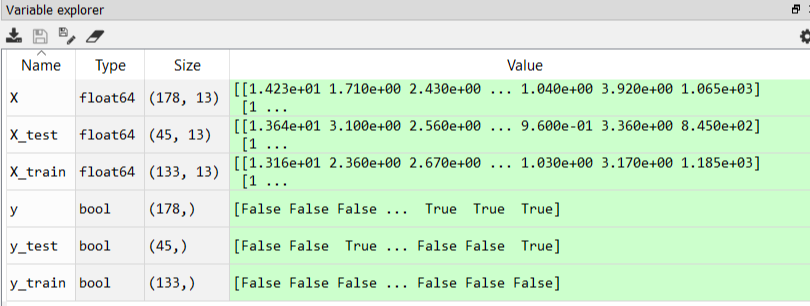
\includegraphics[width=4cm]{figures/1174039/chaptersatu/2.png}
                    \centering
                    \caption{Variable Exploler}
                \end{figure}
            \subsubsection{Mencoba loading an example dataset}
            \begin{enumerate}
                \item mengambil data iris dan digit dari dataset \hfill \break \lstinputlisting[firstline=9, lastline=11]{src/1174039/chaptersatu/no2.py}
                
                \item Menampilkan data digits \hfill \break \lstinputlisting[firstline=13, lastline=13]{src/1174039/chaptersatu/no2.py}
                
                \begin{figure}[H]
                    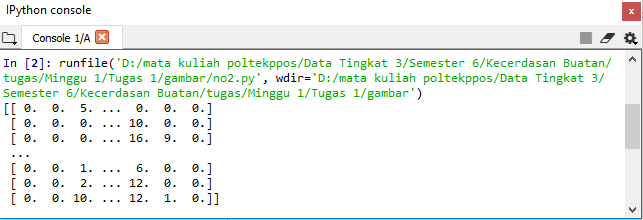
\includegraphics[width=4cm]{figures/1174039/chaptersatu/3.png}
                    \centering
                    \caption{Data Digits}
                \end{figure}

                \item menampilkan digits.target
                \hfill \break \lstinputlisting[firstline=15, lastline=15]{src/1174039/chaptersatu/no2.py}

                \begin{figure}[H]
                    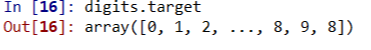
\includegraphics[width=4cm]{figures/1174039/chaptersatu/4.png}
                    \centering
                    \caption{Digits Target}
                \end{figure}

                \item menampilkan data bentuk 2D. \hfill \break \lstinputlisting[firstline=17, lastline=17]{src/1174039/chaptersatu/no2.py}

                \begin{figure}[H]
                    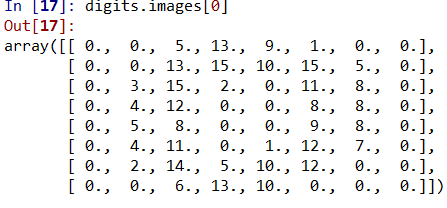
\includegraphics[width=4cm]{figures/1174039/chaptersatu/5.png}
                    \centering
                    \caption{Data 2D}
                \end{figure}
            \end{enumerate}

            \subsubsection{Mencoba Learning and Predicting}
            \hfill \break \lstinputlisting[firstline=1]{src/1174039/chaptersatu/no3.py}

            \subsubsection{Mencoba Model Presistence}
            \hfill \break \lstinputlisting[firstline=1]{src/1174039/chaptersatu/no4.py}

            \subsubsection{Mencoba Conventions}
            \hfill \break \lstinputlisting[firstline=1]{src/1174039/chaptersatu/no5.py}
        \subsection{Penanganan Error}
            \subsubsection{Screenshot Error}
            \begin{figure}[H]
                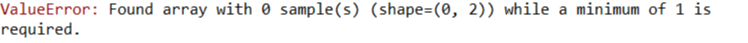
\includegraphics[width=4cm]{figures/1174039/chaptersatu/errorr.png}
                \centering
                \caption{Data 2D}
            \end{figure}
            \subsubsection{Kode error dan jenis error}
            Jenis errornya adalah value error
            \hfill \break \lstinputlisting[firstline=15, lastline=15]{src/1174039/chaptersatu/no3.py}
            \subsubsection{Solusi Error}
            Solusinya adalah dengan menggantikan  nilai nya adalah n\_samples nya agar tidak 0
    \subsection{Cek Plagiarism}
    \begin{figure}[H]
        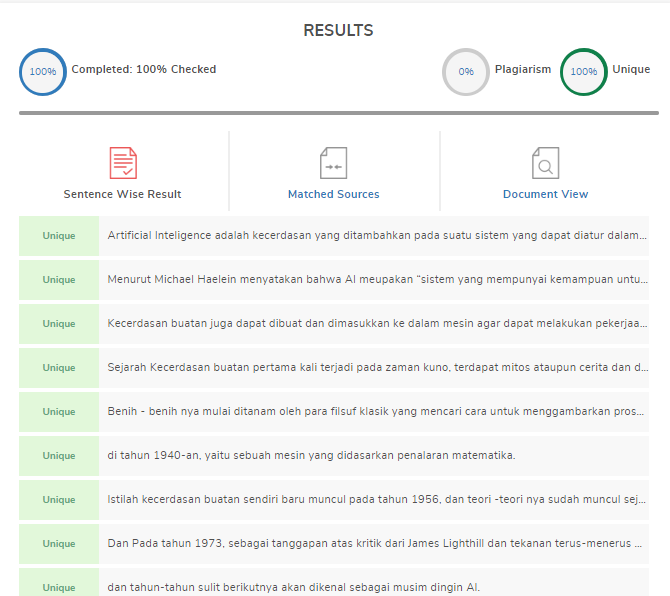
\includegraphics[width=4cm]{figures/1174039/chaptersatu/plagiat.png}
        \centering
        \caption{Cek Plagiarism}
    \end{figure}